\chapter{\LTLf and \LDLf}
\label{logic}
%In this chapter we describe the background knowledge required for this work. We introduce Markov Decision Process (MDP) and Non-Markovian Reward Decision Process (NMRDP), common formalisms in the context of Reinforcement Learning. We describe Linear Temporal Logic over finite traces (\LTLf) and Linear Dynamic Logic over finite traces (\LDLf), that we use for define temporal goal in a RL setting. Then, we describe an important result about RL for NMRDP with \LTLf/\LDLf rewards, that is the basis for this work.

In this chapter we introduce the reader to the main important framework for talk about behaviors over time, which gives the foundations for our approach.
First we talk about the well known Linear time Temporal Logic (\LTL), Propositional Dynamic Logic (\PDL) and their main applications; then we go more in deep by presenting a specific formalism, namely \emph{Linear Temporal Logic over Finite Traces} \LTLf and \emph{Linear Dynamic Logic over Finite Traces} \LDLf.
We require the reader to be acquainted with classical logic \citep{sep-logic-classical} and automata theory \citep{Hopcroft:2000:IAT:557657}.
\section{Linear time Temporal Logic (\LTL)}
\emph{Temporal Logic} \citep{sep-logic-temporal} is a category of formal languages aimed to talk about properties of a system whose truth value might change over time. This is in contrast with atemporal logics, which can only discuss about statements whose truth value is constant. 

\emph{Linear time Temporal Logic} \citep{Pnueli:1977:TLP:1382431.1382534}, or \emph{Linear Temporal Logic} (\LTL) is such a logic. It is the most popular and widely used temporal logic in computer science, especially in formal verification of software/hardware systems, in AI to reasoning about actions and planning, and in the area of Business Process Specification and Verification to specify processes declaratively.

It allows to express temporal patterns about some property $p$, like \emph{liveness} (\emph{$p$ will eventually happen}), \emph{safety} (\emph{$p$ will never happen}) and \emph{fairness}, combinations of the previous patterns (\emph{infinitely often $p$ holds}, \emph{eventually always $p$ holds}).

\subsection{Syntax}
A \LTL formula $\varphi$ is defined over a set of propositional symbols $\Prop$ and are closed under the boolean connectives, the unary temporal operator \Next (\emph{next-time}) and the binary operator $\Until$ (\emph{until}):

\[\begin{array}{rcl}
\varphi &::=& A \mid \lnot \varphi \mid \varphi_1\land \varphi_2 \mid \Next\varphi \mid \varphi_1 \Until \varphi_2
\end{array}
\]
With $A\in \Prop$.

Additional operators can be defined in terms of the ones above: as usual logical operators such as $\OR, \Rightarrow, \Leftrightarrow, \true, \false$ and temporal formulas like \emph{eventually} as $\Diamond \varphi \doteq \true \Until \varphi$, \emph{always} as $\Box \varphi \doteq \lnot \Diamond \lnot \varphi$ and \emph{release} as $\varphi_1 \Release \varphi_2 \doteq \lnot (\lnot \varphi_1 \Until \lnot \varphi_2)$.

\begin{example}\label{ltl-formula-examples}
Several interesting temporal properties can be defined in \LTL:
\begin{itemize}
	\item \emph{Liveness}: $\Diamond \varphi$, which means "condition expressed by $\varphi$ \emph{at some time} in the future will be satisfied", "sooner or later $\varphi$ will hold" or "eventually $\varphi$ will hold". E.g., $\Diamond rich$ (eventually I will become rich), $Request \implies \Diamond Response$ (if someone requested the service, sooner or later he will receive a response).
	\item \emph{Safety}: $\Box \varphi$, which means "condition expressed by $\varphi$, \emph{every time} in the future will be satisfied", "always $\varphi$ will hold". E.g., $\Box happy$ (I'm always happy), $\Box \lnot (temperature >30)$ (the temperature of the room must never be over 30).
	\item \emph{Response}: $\Box \Diamond \varphi$ which means "at any instant of time there exists a moment later where $\varphi$ holds". This temporal pattern is known in computer science as \emph{fairness}.
	\item \emph{Persistence}: $\Diamond \Box \varphi$, which stand for "There exists a moment in the future such that from then on $\varphi$ always holds". E.g. $\Diamond \Box dead$ (at a certain point you will die, and you will be dead forever\footnote{Counterexamples?})
	\item \emph{Strong fairness}: $\Box \Diamond \varphi_1 \implies \Box \Diamond \varphi_2$, "if something is attempted/requested infinitely often, then it will be successful/allocated infinitely often". E.g., $\Box \Diamond ready \implies \Box \Diamond run$ (if a process is in ready state infinitely often, then infinitely often it will be selected by the scheduler).
\end{itemize}
\end{example}

\subsection{Semantics}
The semantics of \LTL is provided by (infinite) \textit{traces}, i.e. $\omega$-word over the alphabet $2^\Prop$. More formally, a \emph{trace} $\trace$ is a \emph{word} on a \emph{path} of a \emph{Kripke structure}.
\begin{definition}[\cite{Clarke:2000:MC:332656}]\label{kripke}
	a Kripke structure $\Kripke$ over a set of propositional symbols $\Prop$ is a 4-tuple $\tup{\States, I, R, L}$ where $\States$ is a finite set of states, $I\subseteq \States$ is the set of initial states, $R \subseteq \States \times \States$ is the transition relation such that $R$ is left-total and $L: \States \to 2^\Prop$ is a labeling function.
\end{definition}
A \emph{path} $\rho$ over $\Kripke$ is a sequence of states $\tup{s_1, s_2, \dots}$ such that $\forall i. R(s_i, s_{i+1})$. From a path we can build a \emph{word} $w$ on the path $\rho$ by  
mapping each state of the sequence with $L$, namely:
\[
w = \tup{L(s_1), L(s_2), \dots}
\]

In simpler words, a trace of propositional symbols $\Prop$ is a infinite sequence of combinations of propositional symbols in $\Prop$. Moreover, we denote by $\trace(i)$ with $i\in\Naturals$ the labels associated to $s_i$, i.e. $L(s_i)$.
\begin{example}
In figure \ref{kripke-example} is depicted an example of Kripke structure $\Kripke$ over $\Prop = \{p, q\}$ where:
\begin{align*}
\States &= \{s_1, s_2, s_3\}\\
I &= \{s_1\}\\
R &= \{(s_1, s_2), (s_2, s_1), (s_2, s_3), (s_3, s_3)\}\\
L &= \{(s_1, \{p, q\}), (s_2, \{q\}), (s_3, \{p\})\}
\end{align*}
 
\begin{figure}[h]
	\centering	
	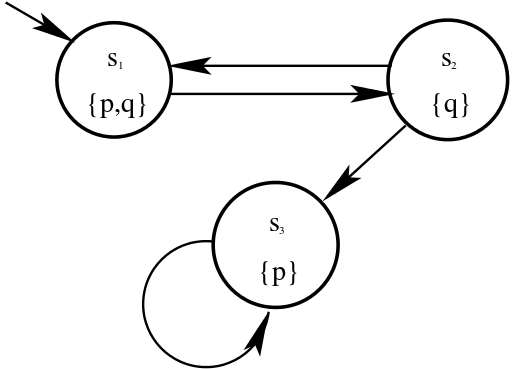
\includegraphics[width=.5\linewidth]{images/KripkeStructureExample}
	\caption{\label{kripke-example}An example of Kripke structure.}
\end{figure}

The path $\tup{s_1, s_2, s_3, s_3, s_3\dots}$ yields the following trace $\trace$:
\begin{align*}
\trace &= \tup{L(s_1), L(s_2), L(s_3), L(s_3), L(s_3),\dots} \\
	&= \tup{\set{p, q}\set{q}, \set{p}, \set{p},\set{p}, \dots}
\end{align*}
\end{example}


\begin{definition}\label{ltl-satisfaction}
	Given a infinite trace $\trace$, we define that a \LTL formula $\varphi$ is \emph{true} at time $i$, in symbols $\trace, i \models \varphi$ inductively as follows:
	\begin{align*}
		\trace, i &\models A \tiff A \in \trace(i)\\
		\trace, i &\models \lnot \varphi \tiff \trace, i \not\models \varphi\\
		\trace, i &\models \varphi_1 \AND \varphi_2 \tiff \trace, i \models \varphi_1 \AND \trace, i \models \varphi_2\\
		\trace, i &\models \Next\varphi \tiff \trace,i+1 \models \varphi\\
		\trace, i &\models \varphi_1 \Until \varphi_2 \tiff \exists j. j\ge i \AND \trace,j \models \varphi \\
	\end{align*}
\end{definition}
Similiarly as in classical logic we give the following definitions:
\begin{definition}
A \LTL formula is \emph{true} in $\trace$, in notation $\trace \models \varphi$, if $\trace, 0 \models \varphi$. A formula $\varphi$ is \emph{satisfiable} if it is true in some $\trace$ and is \emph{valid} if it is true in every $\trace$. $\varphi_1$ \emph{entails} $\varphi_2$, in symbols $\varphi_1 \models \varphi_2$ iff $\forall \trace, \forall i.\trace, i \models \varphi_1 \implies \trace, i \models \varphi_2$.
\end{definition}

Now we state an important result:
\begin{theorem}[\cite{Sistla:1985:CPL:3828.3837}]
	Satisfiability, validity, and entailment for \LTL formulas are \PSPACE-complete.
\end{theorem}
Indeed, Linear Temporal Logic can be thought of as a specific decidable (\PSPACE-complete) fragment of classical first-order logic (\FOL).
\section{Propositional Dynamic Logic (\PDL)}

\subsection{Syntax}
\subsection{Semantics}

\section{Linear Temporal Logic on Finite Traces: \LTLf}
Linear-time Temporal Logic over finite traces, \LTLf, is essentially standard 
\LTL \citep{Pnueli:1977:TLP:1382431.1382534} interpreted over finite, instead of over infinite, traces \citep{de2013linear}.

Indeed, the syntax of \LTLf is the same of \LTLf, i.e. \emph{formulas} of \LTLf are built from a set $\Prop$ of propositional symbols and are closed under the boolean connectives, the unary temporal operator \Next (\emph{next-time}) and the binary operator $\Until$ (\emph{until}):

\[\begin{array}{rcl}
\varphi &::=& \phi \mid \lnot \varphi \mid \varphi_1\land \varphi_2 \mid \Next\varphi \mid \varphi_1 \Until \varphi_2
\end{array}
\]
With $A\in \Prop$.

We use the standard abbreviations:
$\varphi_1\lor\varphi_2 \doteq \lnot(\lnot \varphi_1\land \lnot
\varphi_2)$;
\emph{eventually} as $\Diamond\varphi \doteq \true\Until\varphi$;
\emph{always} as $\Box\varphi \doteq\lnot\Diamond\lnot\varphi$; 
week next $\Wnext\varphi \doteq \lnot\Next\lnot\varphi$ (note that on finite
traces $\lnot\Next\varphi \not\equiv \Next\lnot\varphi$); and $Last \doteq \Wnext\false$ denoting the end of the trace. 

Formally, a \emph{finite trace} $\trace$ is a finite word over the alphabet $2^\Prop$, i.e. as alphabet we have all the possible propositional interpretations of the propositional symbols in $\Prop$. For the semantics we refer to \citep{de2013linear}.

\LTLf is as expressive as 
first-order logic (\FO)
over finite traces
and star-free regular expressions (\REGEX).
\section{Regular Expression (\REGEX)}
\section{Linear Dynamic Logic on Finite Traces: \LDLf}
\LDLf, \emph{Linear Dynamic Logic of Finite Traces} merges \LTLf with \REGEX$_f$ (\REGEX on finite traces) in a very natural way.
The logic is called LDL f
\LTLf can be extended to 


 which is expressive as monadic second-order logic 
(\MSO) over finite traces \citep{de2013linear}.

Linear Dynamic Logic of Finite
Traces

Formally, \LDLf formulas $\varphi$ are built as follows:
%%%
\[\begin{array}{lcl}
\varphi &::=& \ttrue  \mid \lnot \varphi \mid \varphi_1 \land \varphi_2 \mid \DIAM{\varrho}\varphi \\
\varrho &::=& \phi \mid \varphi? \mid  \varrho_1 + \varrho_2 \mid \varrho_1; \varrho_2 \mid \varrho^*
\end{array}
\]
%%%
where $\ttrue$ stands for logical true; $\phi$ is a propositional
formula over $\Prop$; $\varrho$ denotes path expressions, which are \REGEX over
propositional formulas $\phi$ with the addition of the test construct
$\varphi?$ typical of \PDL.  We use abbreviations
$\BOX{\varrho}\varphi\doteq\lnot\DIAM{\varrho}{\lnot\varphi}$ as in \PDL.
Intuitively, $\DIAM{\varrho}\varphi$ states that, from the current step
in the trace, there exists an execution satisfying the \REGEX $\varrho$ 
such that its last step satisfies $\varphi$, while
$\BOX{\varrho}\varphi$ states that, from the current step, all executions
satisfying the \REGEX $\varrho$ are such that their last step
satisfies $\varphi$.
%%
Tests are used to insert into the execution path checks for
satisfaction of additional \LDLf formulas.
%
%
%%%

Given an \LTLf/\LDLf formula $\varphi$,
we can construct a deterministic finite state automaton (\DFA) \citep{RaSc59} 
$\automaton_\varphi$ that tracks satisfaction of $\varphi$, 
given a finite trace
%~\footnote{An analogous transformation to automata applies to several other formalisms for representing non-Markovian rewards \cite{BBG96,ThiebauxGSPK06,Slaney05,Gretton07,Gretton14,LacerdaPH14,LacerdaPH15}. All results presented here apply to those formalisms as well.},

accepting a sequence of propositional interpretations {\em
	iff} the sequence satisfies $\varphi$. This construction
is a key element in the efficient transformation from non-Markovian
rewards to Markovian rewards over an extended MDP \citep{BDP-AAAI18}.
%%%
%
The idea is to use \LTLf/\LDLf formulas to specify when sequences of 
state-action pairs, rather than one pair only, should be rewarded.
Notice that we can easily incorporate the executed action in the current state
by using propositions. In this way, we can make \LTLf/\LDLf deal with 
actions, as well. From now on, we assume this is the case.

\section{\LTLf and \LDLf translation to automata}
Both \LTLf and \LDLf can be directly translated into alternating automata on words (\AFW). Formally, an 



delta function for the NFA:
\begin{align}
\begin{aligned}
\Dfun{\ttrue} 			\ind &= \ind \true\\
\Dfun{\ffalse} 			\ind &= \ind \false\\
\Dfun{\PropFormula}   	\ind &= \ind a\\
\Dfun{\varphi_1 \AND \varphi_2} 			\ind &= \ind   \Dfun{\varphi_1} \AND \Dfun{\varphi_2}\\
\Dfun{\varphi_1 \OR  \varphi_2} 			\ind &= \ind   \Dfun{\varphi_1} \OR \Dfun{\varphi_2}\\
\Dfun{\DIAM{\PropFormula}\varphi}             \ind &= \ind 
	\begin{cases}
		\textbf{\textit{E}}(\varphi) 	& \text{if}\ \PropInt \models \PropFormula\\
		\false     						& \text{if}\ \PropInt \not\models \PropFormula\\
	\end{cases}\\
\Dfun{\DIAM{\regexp?}\varphi}             			\ind &= \ind \Dfun{\regexp} \AND \Dfun{\varphi}\\
\Dfun{\DIAM{\regexp_1 + \regexp_2}\varphi}             \ind &= \ind \Dfun{\DIAM{\regexp_1}\varphi} \OR \Dfun{\DIAM{\regexp_2}\varphi}\\
\Dfun{\DIAM{\regexp_1 ; \regexp_2}\varphi}             \ind &= \ind \Dfun{\DIAM{\regexp_1}\DIAM{\regexp_2}\varphi}\\
\Dfun{\DIAM{\regexp^*}\varphi}             			\ind &= \ind \Dfun{\varphi} \OR \Dfun{\DIAM{\regexp}\FalseDelta{\DIAM{\regexp^*}\varphi}}\\
\Dfun{\BOX{\PropFormula}\varphi}             \ind &= \ind 
	\begin{cases}
		\textbf{\textit{E}}(\varphi) 	& \text{if}\ \PropInt \models \PropFormula\\
		\true     						& \text{if}\ \PropInt \not\models \PropFormula\\
	\end{cases}\\
\Dfun{\BOX{\regexp?}\varphi}             			\ind &= \ind \Dfun{\nnf(\NOT \regexp)} \OR \Dfun{\varphi}\\
\Dfun{\BOX{\regexp_1 + \regexp_2}\varphi}             \ind &= \ind \Dfun{\BOX{\regexp_1}\varphi} \AND \Dfun{\BOX{\regexp_2}\varphi}\\
\Dfun{\BOX{\regexp_1 ; \regexp_2}\varphi}             \ind &= \ind \Dfun{\BOX{\regexp_1}\BOX{\regexp_2}\varphi}\\
\Dfun{\BOX{\regexp^*}\varphi}             			\ind &= \ind \Dfun{\varphi} \AND \Dfun{\BOX{\regexp}\TrueDelta{\DIAM{\regexp^*}\varphi}}\\
\Dfun{\TrueDelta{\psi}} 			\ind &= \ind \true\\
\Dfun{\FalseDelta{\psi}} 			\ind &= \ind \false\\
\end{aligned}					
\end{align}





